%Dokumententyp
\documentclass[a4paper]{article}


\usepackage[a4paper,left=2cm, right=3cm, top=2cm]{geometry}

%Kodierung
\usepackage[utf8]{inputenc}
\usepackage[T1]{fontenc}

%Grafiken einbinden
\usepackage{graphicx}
\usepackage{subfigure} 

%Position von Grafiken und Tabellen erzwingen:
\usepackage{float}

%URLs im Literaturverzeichnis
\usepackage{url}

\usepackage{amsmath}

%Vektoren einfacher angeben:
\newcommand{\vektor}[1]{\left( \begin{array}{c} #1 \end{array} \right) }


%Schriftart Arial:
% \usepackage{helvet}

%Figures with text around it:
\usepackage{wrapfig}

\usepackage{listings}

%seitennummern rechts:
% \usepackage{fancyhdr}
% \fancyhf{} % clear all header and footers
% \renewcommand{\headrulewidth}{0pt} % remove the header rule
% \rfoot{\thepage}
% \fancypagestyle{plain}{%redefining plain pagestyle
% \fancyhf %clear all headers and footers fields
% \fancyhead[R]{\thepage} %prints the page number on the right side of the header
% }

%Schriftart Times New Roman "like"
\usepackage{txfonts}

%Sprache
\usepackage[german]{babel}

%Checkmarks: (usage: \checkmark)
\usepackage{dingbat}

\usepackage{listings}
\usepackage{color}
\definecolor{javared}{rgb}{0.6,0,0} % for strings
\definecolor{javagreen}{rgb}{0.25,0.5,0.35} % comments
\definecolor{javapurple}{rgb}{0.5,0,0.35} % keywords
\definecolor{javadocblue}{rgb}{0.25,0.35,0.75} % javadoc
 
\lstset{language=Java,
basicstyle=\ttfamily,
keywordstyle=\color{javapurple}\bfseries,
stringstyle=\color{javared},
commentstyle=\color{javagreen},
morecomment=[s][\color{javadocblue}]{/**}{*/},
numbers=left,
numberstyle=\tiny\color{black},
stepnumber=1,
numbersep=5pt,
tabsize=4,
showspaces=false,
lineskip={-1.5pt},
showstringspaces=false}

%Tabellenextras
\usepackage{tabularx}

%Zeilenabstand 1.5
\linespread{1.5}
\usepackage{setspace}

%Figure Captions mit Fußnoten
\usepackage{footnote}
%\setlength{\parindent}{0pt} 


%itemize items richtig ausrichten (nicht links überlappen!)
% \setlist{leftmargin=0}

% %%%%TITELSEITE%%%%%%(
% \title{ Konzept und Implementierung\\ eines Systems zur \\Anforderung und Verwaltung von virtuellen privaten Clustern}
% \author{\textbf{\large Bachelorarbeit}}
% 
% \date{zur Erlangung des akademischen Grades Bachelor of Science an der Universität Paderborn im Fachbereich Informatik im Studiengang Bachelor Informatik}

% %%%%TITELSEITE%%%%%%)

% \pagestyle{fancy}
\begin{document}

\title{Algorithmische Geometrie - Sommersemester 2015\\
       5. Aufgabenblatt }
\author{Simon Koennecke und Felix Bröker}
\date{}
\maketitle

\section*{Aufgabe 1 - Suchen in ebenen Unterteilungen}
\subsection*{Aufbau einer Datenstruktur}
Annahme: Es ist der ebene Graph $G$ gegeben. 

Wir konstruieren im Folgenden auf Basis von $G$ eine Directed Acyclic Graph (DAG)-Struktur $S$, mittels derer 
später in $\mathcal{O}(\log n)$ ermittelt werden kann, in welcher Facette/Dreieck des Graphen
sich ein Punkt $p$ befindet:

$S_i$ sei die Triangulierung der verbliebenen Punkte vom Graphen $G$ im Verarbeitungsschritt $i$.

Zu Beginn gilt: $i = 0$ und $S_i$ = $G$.

\begin{enumerate}
 \item Solange $S_i$ kein Dreieck
 \begin{enumerate}
  \item Setze $S_{i+1} = S_i$
  \item Finde eine unabhängige Knotenmenge $U_i$ von $S_i$, wobei jeder Knoten der Menge, innerer Knoten mit Grad $< 12$ ist.
  \item Solange $U_i$ nicht leer
  \begin{enumerate}
   \item Enferne beliebigen Knoten $u \in U_i$ aus $S_{i+1}$. Benenne die hiermit entfallenen Dreiecke als $\Delta_{alt}$
   \item Trianguliere die Nachbarschaft von $u$ in $S_{i+1}$ neu. Benenne die neu entstandenen Dreiecke als $\Delta_{neu}$.
   \item Die Verbindungen zwischen $S_i$ und $S_{i+1}$ werden entsprechend der Kantenmenge
   
   $\left\{(\delta_{neu}, \delta_{alt}) \quad|\quad (\delta_{neu} \in \Delta_{neu}, \delta_{alt} \in \Delta_{alt} \right\}$ konstruiert.
   (Die Kardinalität der Kantenmenge kann in bestimmten Fällen auch noch weiter reduziert werden)
  \end{enumerate}
  \item Setze $i = i + 1$
 \end{enumerate}

\end{enumerate}

Um die Vorverarbeitungs-, Anfragezeit sowie Speicherplatz abschätzen zu können, greifen wir auf folgende Überlegungen zurück:

\begin{itemize}
\item Auf jeder Ebene $S_i$ mit $i > 0$ gilt: Alle Dreiecke $\delta_{neu}$ haben jeweils maximal 11 Zeiger auf Dreiecke aus $\Delta_{alt}$. Dies folgt direkt aus der Eigenschaft der unabhängigen Knotenmenge, welche nur Knoten mit Grad $ < 12$, also maximal Grad 11, beinhaltet. 

\item $|U_i| \geq \frac{n}{24} - \frac{1}{6}$, d.h. die Menge $U_i$ umfasst mindestens $\frac{n}{24} - \frac{1}{6}$ unabhängige Knoten und somit werden im $i$-ten Durchlauf auch mindestens $\frac{n}{24} - \frac{1}{6}$ Knoten der Triangulierung $S_{i+1}$ gelöscht. Dies folgt aus den Eigenschaften der unabhängigen Menge und der Triangulierung. Da die Menge $U_i$ aus der Menge der Knoten mit Grad $< 12$
durch das Löschen von angrenzenden Knoten konstruiert wird und diese die Größe $\geq \frac{n}{2}-2$ besitzt, müssen am Ende $\geq \frac{\frac{n}{2}-2}{12} = \frac{n}{24} - \frac{1}{6}$ Knoten als Menge $U_i$ "`übrig bleiben"'.

\item Die Höhe von $S$ lässt sich mit $\mathcal{O}(\log n)$ abschätzen. Denn, wenn sich die Knotenzahl
pro Ebene $S_i$ (wie im vorigen Schritt genannt) um mindestens $\frac{n}{24} - \frac{1}{6}$ verringert, so bleiben höchstens $n - (\frac{1}{24} n - \frac{1}{6}) = \frac{23}{24} n + \frac{1}{6}$ Knoten in
der nächsten Ebene über. 

Angenommen, $k$ sei die Höhe von $S$, dann gilt mit wiederholtem Einsetzen (auf Höhe k besitzt $S_k$ nur noch 3 Knoten): 

$(\frac{23}{24})^k n + \frac{1}{6} \sum_{i = 0}^{k-1} (\frac{23}{24})^i = 3 
\Leftrightarrow 
(\frac{23}{24})^k n + \frac{1}{6} \frac{1-(\frac{23}{24})^k}{1- \frac{23}{24}} = 3
\Leftrightarrow 
(\frac{23}{24})^k n + \frac{1-(\frac{23}{24})^k}{6- \frac{138}{144}} = 3
\Leftrightarrow 
(\frac{23}{24})^k (6- \frac{138}{144}) n + 1-(\frac{23}{24})^k = 3 (6- \frac{138}{144})
\Leftrightarrow 
(\frac{23}{24})^k ((6- \frac{138}{144}) n - 1) = 3 (6- \frac{138}{144}) - 1
\Leftrightarrow 
(\frac{23}{24})^k = \frac{3 (6- \frac{138}{144}) - 1}{((6- \frac{138}{144}) n - 1) }
\Leftrightarrow 
k = \log_{\frac{23}{24}}\frac{3 (6- \frac{138}{144}) - 1}{((6- \frac{138}{144}) n - 1) }
= \mathcal{O}(\log n).
$

\end{itemize} 

\subsection*{Vorverarbeitungszeit}
Aufgrund der berechneten Höhe von $S = \mathcal{O}(\log n)$, wird "`1"'  $\mathcal{O}(\log n)$ mal ausgeführt. Die einzelnen Teilschritte lassen sich wie folgt einordnen:

\begin{itemize}
\item[(a)] Das "`Kopieren"' von $S_i$ benötigt $\mathcal{O}(n)$ Zeit.
\item[(b)] Das Finden einer unabhängigen Knotenmenge $S_i$ ist in $\mathcal{O}(n)$ Zeit möglich.
\item[(c)] Dieser Schritt wird $\mathcal{O}(n)$ mal ausgeführt. Wie wir festgestellt haben, 
           ist die Menge der neu entstehenden Dreiecke pro Schritt,
           sowie folglich der Aufwand für das Neu-Triangulieren der Nachbarn pro Schritt konstant.
           Insgesamt benötigt (c) damit $\mathcal{O}(n)$ Zeit.
\item[(d)] Das Heraufsetzen der Indexvariable $i$ benötigt konstante Zeit.
\end{itemize}

Damit haben wir eine Gesamtlaufzeit für die Vorverarbeitung von $\mathcal{O}(\log n) (\mathcal{O}(n) +
\mathcal{O}(n) + \mathcal{O}(n) + \mathcal{O}(1)) = \mathcal{O}(n \log n)$.

\subsection*{Anfragezeit}
Die Anfragezeit liegt entsprechend der Höhe der DAG-Struktur $S$ in $\mathcal{O}(\log n)$.

\subsection*{Speicherplatzbedarf}
Die Ebene $S_i$ hat einen Speicherplatzbedarf von $\mathcal{O}(n)$.
Damit liegt der gesamte Speicherplatzbedarf in $\mathcal{O}(n \log n)$.

\section*{Aufgabe 2 - $L_1$-Voronoi-Diagramme}

Um einen ersten Eindruck zu bekommen, betrachten wir den Bisektor zweier beliebiger Punkte $a, b \in \mathcal{R}^2$. Diese seien in $x$-Richtung aufsteigend sortiert. 

Für die Gestalt des Bisektors gibt es folgende mögliche Fälle:
\begin{enumerate}
	\item $a = b$ : Wenn $a$ und $b$ identisch sind, entspricht der Bisektor dem gesamten $\mathcal{R}^2$.
	\item $a$ und $b$ kollinear : Wenn $a_x = b_x$ oder $a_y = b_y$, dann ist der Bisektor genau durch deren Mittelsenkrechte gegeben. 
	\item $|a_x - b_x| = |a_y - b_y|$ : Wenn $a$ und $b$ sowohl in $x$- als auch in $y$-Richtung 
	den gleichen Abstand haben, ist der Bisektor durch die Flächen 
	$F_1 = \left \{\vektor{a_x \\ b_y} + \lambda \vektor{-1 \\ 0} + \mu \vektor{0 \\ b_y - a_y} \quad |   \lambda, \mu \in \mathcal{R}  \geq 0 \right\}$ , 
	
	$F_2 = \left \{\vektor{b_x \\ a_y} + \lambda \vektor{1 \\ 0} + \mu \vektor{0 \\ a_y - b_y} \quad |   \lambda, \mu \in \mathcal{R}  \geq 0  \right \}$
	und die Strecke
	$S = \overline{(a_x, b_y) (b_x, a_y)}$ gegeben (siehe Beispiel in Abb. (a)). 
	\item In allen anderen Fällen ist der Bisektor durch eine Strecke $S$ mit der Steigung 1 bzw. -1 und
	zwei Strahlen $R_1, R_2$ gegeben (siehe Beispiele in Abb. (b),(c)).
	
	Der Mittelpunkt von $S$ ist gegeben mit $P = (\frac{a_x + b_x}{2}, \frac{a_y + b_y}{2})$, die Steigung von $S$ mit $m = \frac{a_y - b_y}{|a_y - b_y|}$. Damit ist die Strecke $S$ beschrieben durch
	$\overline{(P_x + m (b_y - P_y), b_y) (P_x - m (b_y - P_y), a_y)}$, falls $|b_y - a_y| < |b_x - a_x|$
	, ansonsten durch
	$\overline{(a_x, P_y + m (a_x - P_x)) (b_x, P_y - m (a_x - P_x))}$. 
	
	Die Strahlen $R_1$ und $R_2$ sind im Fall $|b_y - a_y| < |b_x - a_x|$ durch $R1 = \left \{\vektor{P_x + m (b_y - P_y) \\ b_y} + \lambda \vektor{0 \\ -m}   \quad |   \lambda \in \mathcal{R}  \geq 0  \right \}$ und $R2 = \left \{\vektor{P_x - m (b_y - P_y)\\ a_y} + \lambda \vektor{0 \\ m}   \quad |   \lambda \in \mathcal{R}  \geq 0  \right \}$, ansonsten durch $R1 = \left \{\vektor{a_x \\ P_y + m (a_x - P_x)} + \lambda \vektor{m \\ 0}   \quad |   \lambda \in \mathcal{R}  \geq 0  \right \}$ und $R2 = \left \{\vektor{b_x\\ P_y - m (a_x - P_x)} + \lambda \vektor{-m \\ 0}   \quad |   \lambda \in \mathcal{R}  \geq 0  \right \}$ gegeben. 
	
\end{enumerate}

Wie zu sehen ist, bestehen die $L_1$-Kanten in den meisten Fällen aus Kurven , welche aus einem horizontalen/vertikalen Strahl, einer Strecke der Steigung 1/-1 und einem weiteren horizontalen/vertikalen Strahl zusammengesetzt sind. Allerdings können wie im ersten oder dritten Fall 
auch ganze ("`unendliche"') Flächen Teil der Voronoi-Kanten sein. Die folgenden Abbildungen illustrieren
ein paar beispielhafte Fälle eines $L_1$-VDs.


\begin{figure} [htbp] 
	\subfigure[Bisektor der Punkte (0,0), (1,1)]{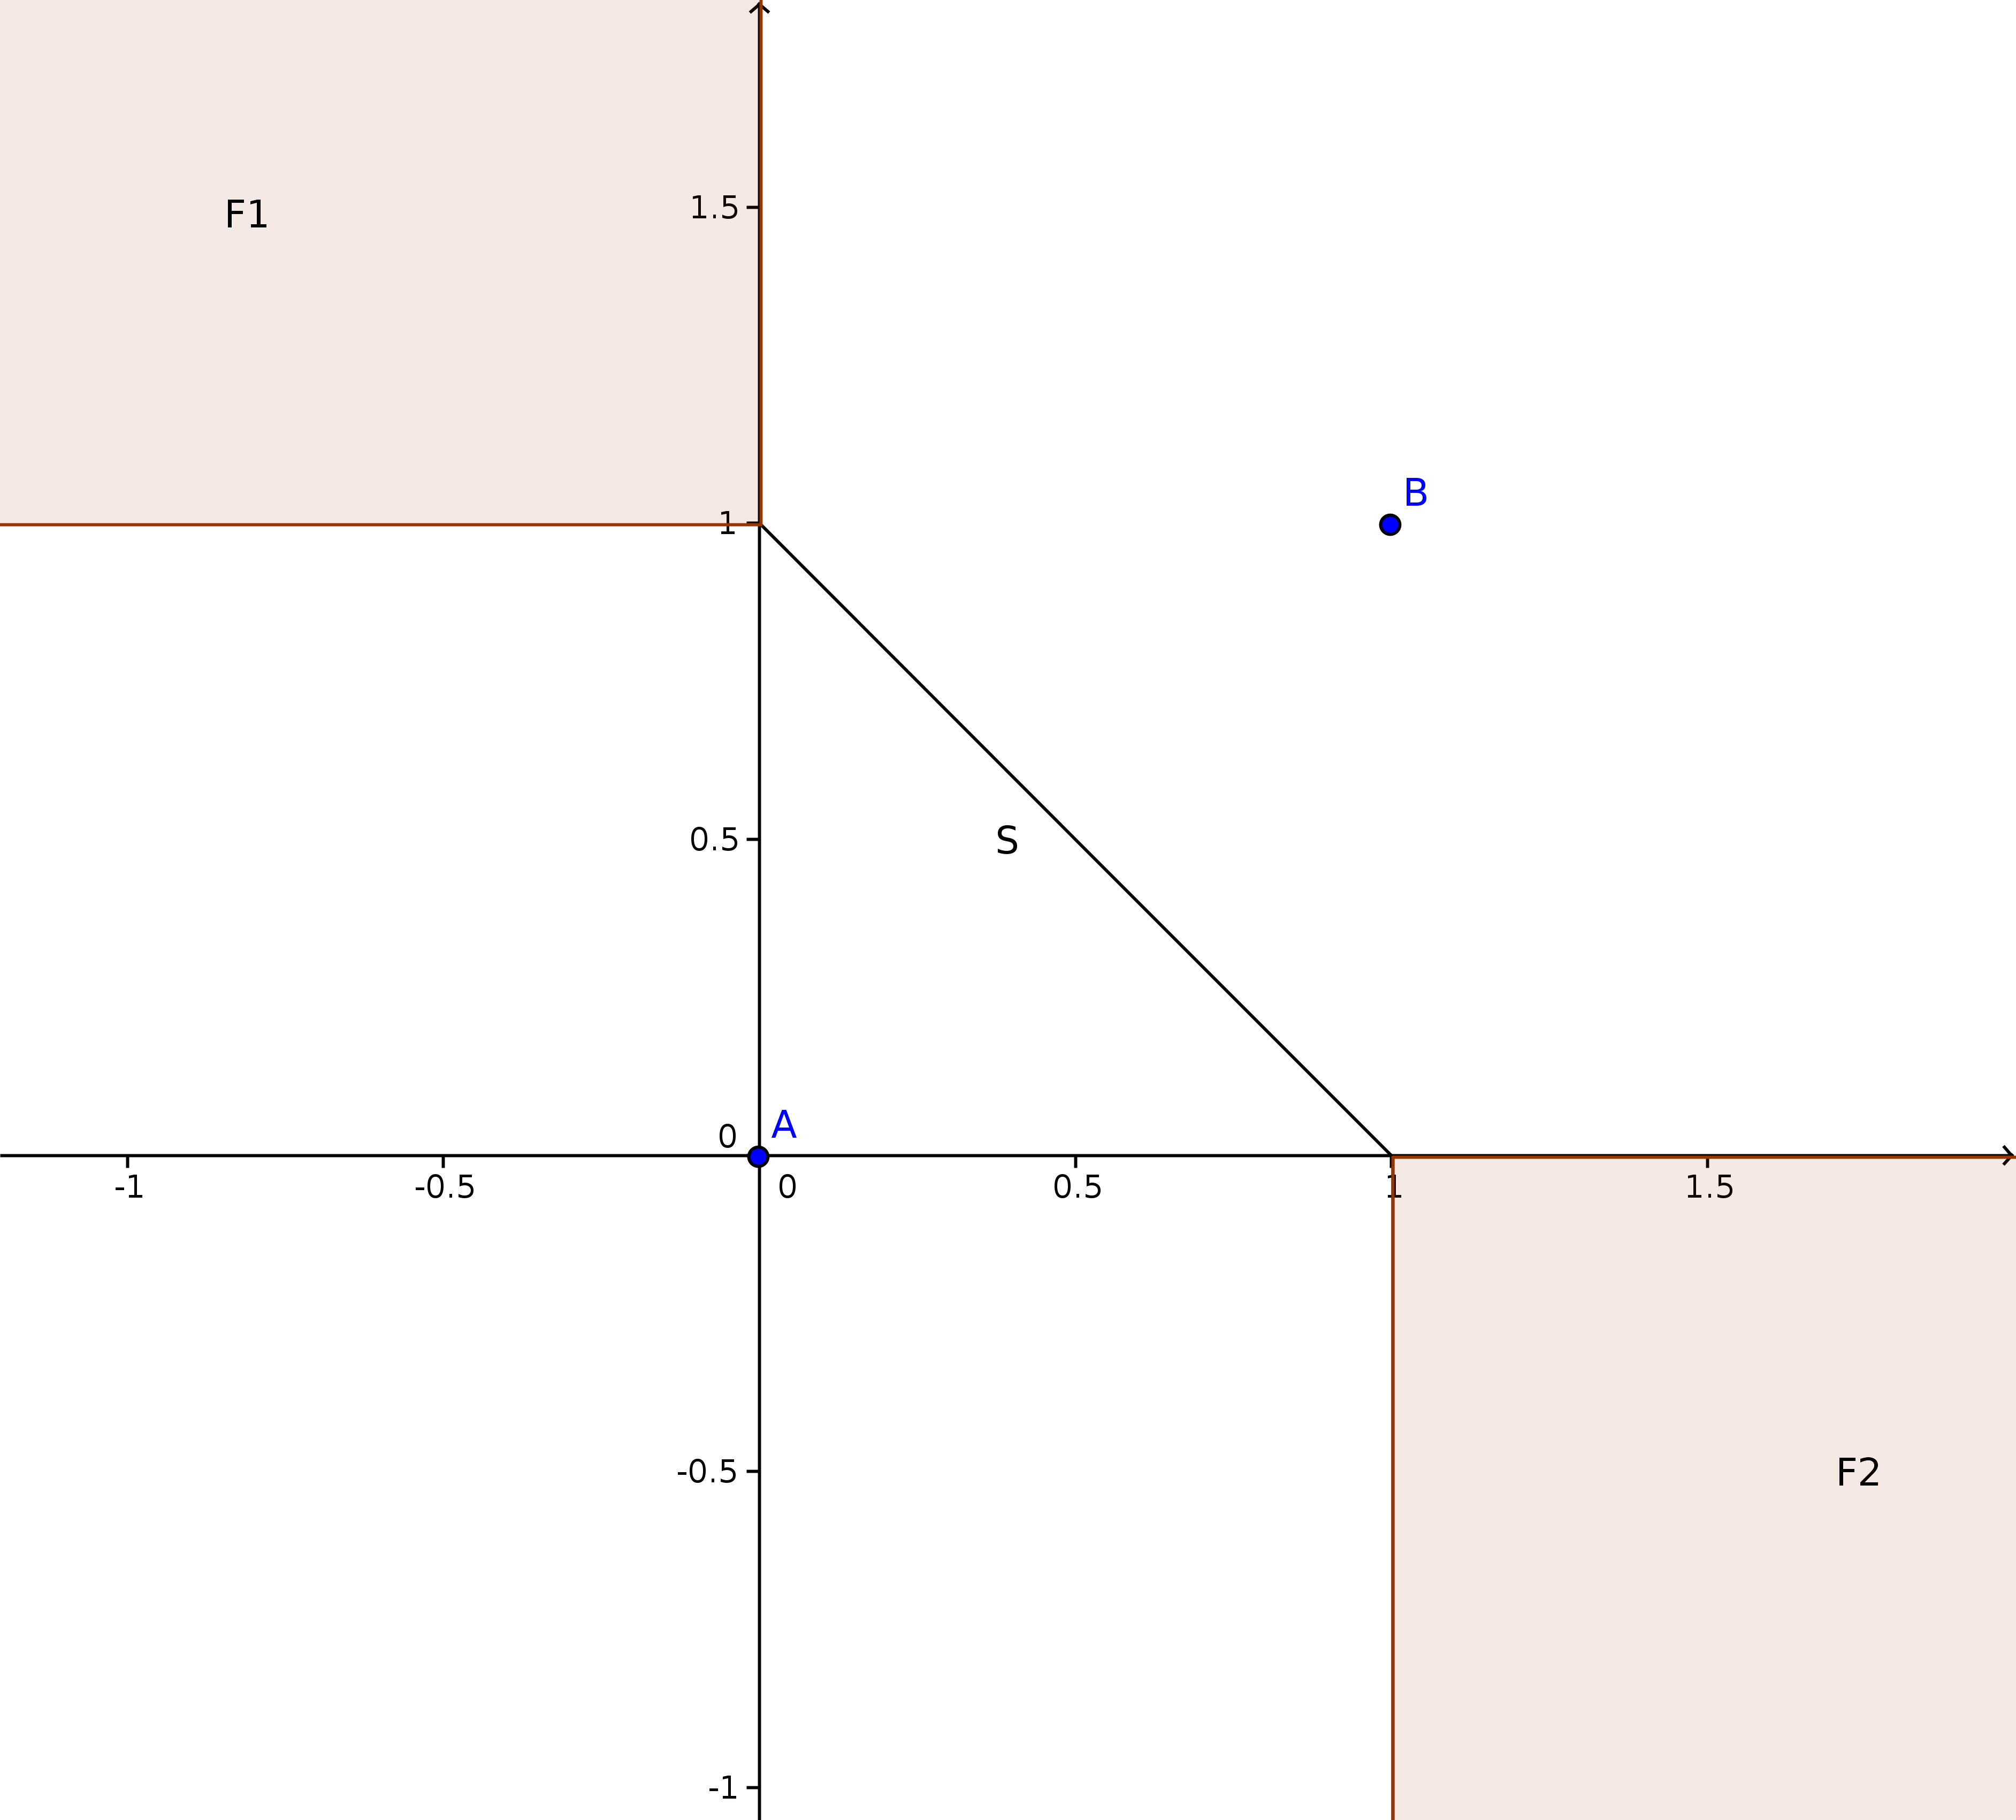
\includegraphics[width=0.5\textwidth]{bisector1}}
	\subfigure[Bisektor der Punkte (0,0), (2,1)]{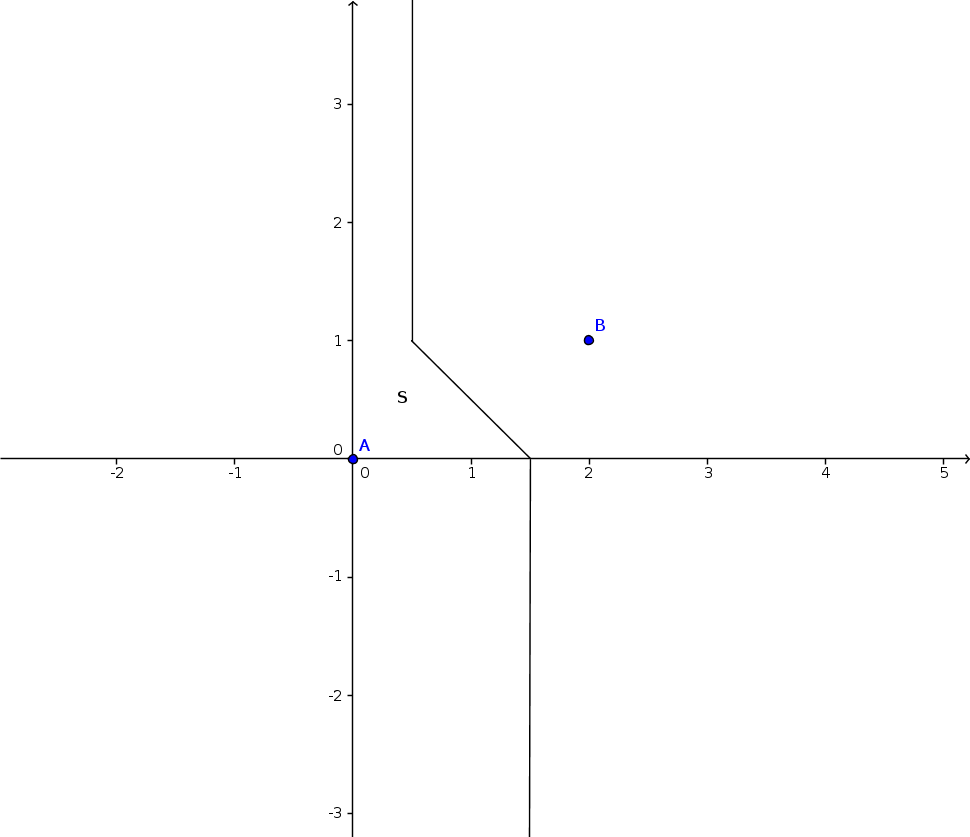
\includegraphics[width=0.5\textwidth]{bisector2}}
	\subfigure[Bisektor der Punkte (0,2), (1,0)]{\includegraphics[width=0.5\textwidth]{bisector3}}
    \subfigure[Voronoi-Diagramm (Manhattan-Distance) - Beispiel 1]{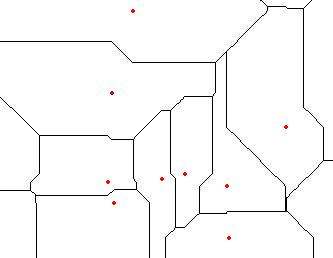
\includegraphics[width=0.5\textwidth]{01.jpg}} 
    \subfigure[Voronoi-Diagramm (Manhattan-Distance) - Beispiel 2]{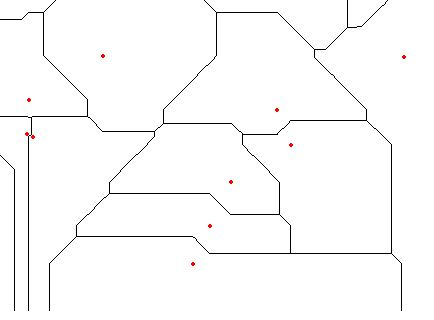
\includegraphics[width=0.5\textwidth]{02.jpg}} 
    \subfigure[Voronoi-Diagramm (Manhattan-Distance) - Beispiel 3]{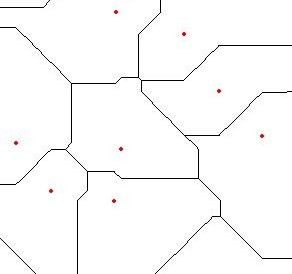
\includegraphics[width=0.5\textwidth]{03.jpg}} 
%\caption{test}
\label{test} 
\end{figure} 

\section*{Aufgabe 3 - Suche in ebenen Unterteilungen - Verallgemeinerung}





\end{document}
